\documentclass[two column]{article}
\usepackage[utf8]{inputenc}

\usepackage{amsmath,amsthm,amssymb}

\usepackage{subcaption}
\usepackage{graphicx}

\usepackage{diagbox}

\graphicspath{{./../images/}}

\usepackage{listings}


\usepackage{color}

\definecolor{gray}{rgb}{0.5,0.5,0.5}
\definecolor{orange}{rgb}{0.8,0,0}

\lstdefinestyle{ccode}{
  belowcaptionskip=1\baselineskip,
  breaklines=true,
  frame=L,
  xleftmargin=\parindent,
  language=C,
  showstringspaces=false,
  basicstyle=\footnotesize\ttfamily,
  keywordstyle=\bfseries\color{green},
  commentstyle=\color{gray},
  identifierstyle=\color{blue},
  stringstyle=\color{orange},
}

\def\listingsfont{\ttfamily} 
\def\listingsfontinline{\ttfamily}

\title{Report for computer exercise 1 - Filter in MPI}
\author{Anton Karlsson\\antka388\\931217-7117}
\date{}
\begin{document}
\maketitle

\section{Code description}
\label{sec:code-description}
An over-view of the two filters used in lab. In both filters, MPI was
intiliasized and the master process read the input image, which could
then be scattered to the other processes in the communication
world. However, they where sent in some different ways due to data
dependecies.

Let $n$ denoted the problem size (i.e the number of pixels), and $p$ 
the number of processors used.  

\subsection{Blur filter}
\label{sec:blur-filter}

In the blur filter, each process needed to have access to pixels in a
radius around the chunk of its imgae that have been sent from the
master process. Along with this and the fact that the image was read as
long string, rather than a 2 by 2 matrix, Each process recvied $n/p$
number of rows of pixels that is to be written by the process, along
with some extra \texttt{radius}  number of rows of pixels, from above
and below. Note that the processes that had chunks of the middle part
of the image recived extra pixels from above and below chunks of
images.

After that, each process could apply the blurfilter on its private
chunk of pixels, and then the master process gather the result and
computed the ouputfile.

\subsection{Threshold filter}
\label{sec:threshold-filter}

The threshold filter did not need the overlap of pixels, so the master
process can simply scatter $n/p$ rows of pixels to each process. Then,
each process can comute the pixel mean from its chunk. After that, the
master process perfomes a reduce communication with where it compute
the mean for each process, thus obtaining an global threshold
parameter, which can brodacsted to all process, which they can use to
compute the threshold filter on there individual chunk. From there,
individual chunks is gather by the master process, which can then
create the output file.

\section{Results}
\label{sec:results}

The results are splited up into to subsection; one covering the
elapsed times and comparing the time when using more processors, the
other section covers the images that was produced. 

\subsection{Computational results}
\label{sec:comp-results}

A comparision of effecitenty of the number of processors used is shown
in Table \ref{tab:1} for the blur filter (with a radius of 50), and Table \ref {tab:2} for
the threshold filter. The problem size, i.e. the number of pixels used,
is denoted by $n$, and the number of processors used is denoted by $p$.


\begin{table}[h]
  \centering
  \begin{tabular}[]{c|c|c|c}
    \backslashbox{$p$}{$n$} & 515788 & 1048576 & 9000000 \\
    \hline 
    1 & 2.51599  & 4.69139  & 40.1536 \\
    2 & 1.36332  & 2.5482  & 20.7491 \\
    4 & 0.850465  & 1.59503 & 12.8175 
  \end{tabular}
  \caption{Elapsed time when differrent number of processors was used.}
  \label{tab:1}
\end{table}

\begin{table}[h]
  \centering
  \begin{tabular}[h]{c|c|c|c}
    \backslashbox{$p$}{$n$} & 515788 & 1048576 & 9000000\\
    \hline 
    1 & 0.0421069 & 0.0667911 & 0.431706   \\
    2 & 0.0100501  & 0.0175579 & 0.282922   \\
    4 & 0.00811195 & 0.0438762 & 0.105303
  \end{tabular}
  \caption{Elapsed time when diferrent number of processors was used
    for the threshold filter}
  \label{tab:2}
\end{table}

\subsection{Filter results}
\label{sec:filter-results}

The result of using \texttt{im1.png} is shown in Figure
\ref{fig:thres}. 

\begin{figure}[h]
  \centering
  \begin{subfigure}{0.3\textwidth}
    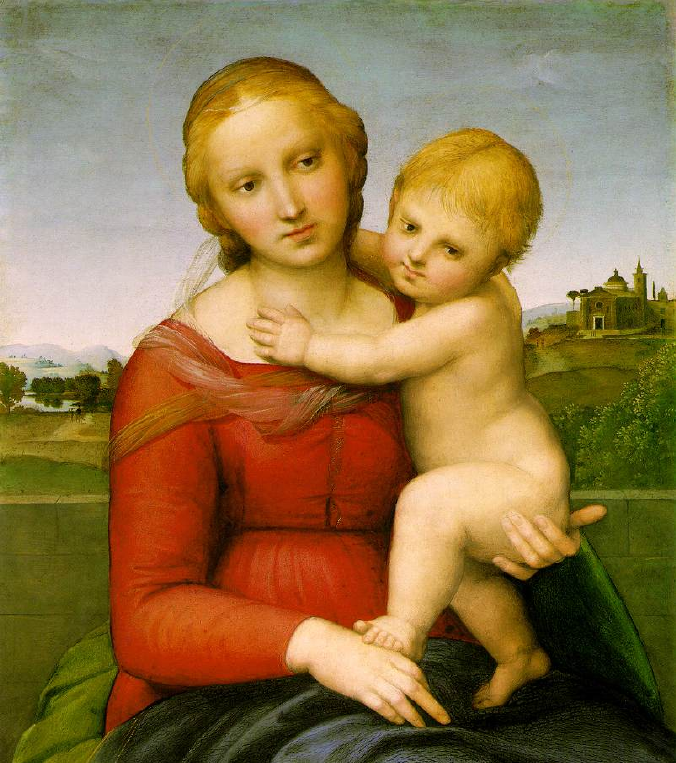
\includegraphics[width=\textwidth]{im1.png}
    \caption{Before filtering.}
  \end{subfigure}
  ~%
  \begin{subfigure}{0.3\textwidth}
    
\includegraphics[width=\textwidth]{im1test.png}
    \caption{After the blurfilter with radius $r = 50$.}
  \end{subfigure}
  ~%
  \begin{subfigure}{0.3\textwidth}
    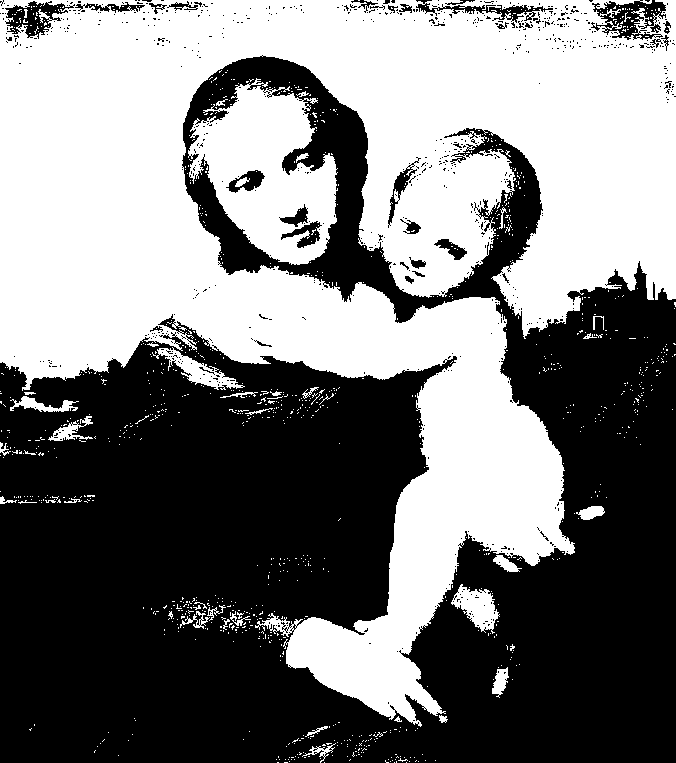
\includegraphics[width=\textwidth]{test.png}
    \caption{After the threshold filter.}
  \end{subfigure}
  \caption{Image result using the threshold filter and the blurfilter
    (with a radiues $r = 50$) on 
    \texttt{im1.png}. Before and after}
  \label{fig:thres}
\end{figure}



\clearpage
\onecolumn
\section*{Code}
\label{sec:code}

\lstinputlisting[caption=blurmain.c, style=ccode]
{../blurmain.c}

\clearpage

\lstinputlisting[caption=thresmain.c, 
style=ccode]{../thresmain.c}




\end{document}

%%% Local Variables:
%%% mode: latex
%%% TeX-master: t
%%% End:
